\chapter{MeVガンマ線天文学}
%天文学は色々な波長のよる観測で進んできた
かつてから可視光から電波・赤外線・X線と様々な波長の電磁波の観測は天文学の発展に貢献してきた。さらに今日では陽子を主とする宇宙線やニュートリノなどの観測も行われる様になり、観測によって得られる宇宙の情報はより豊かになった。

%ガンマ線天体観測と色々な波長について
宇宙の情報を得る手段の一つにガンマ線の観測がある。ガンマ線とは数百keV以上のエネルギーを持つ電磁波を指す。1950年代に早川らにより、宇宙線と星間物質との相互作用で作られる$\pi^{0}$中間子の崩壊によってガンマ線が放射されることが予言されて以来1967年にOSO-3($\geq$ 50$\ $kev)、1972年にSAS-2(20\ MeV $\sim$ 1$\ $GeV)、1975年にCOS-B(2 $\ $keV $\sim$ 5$\ $GeV)と、次々とガンマ線観測衛星が打ち上げられ、多くのガンマ線天体を発見している。また、sub-MeV$\sim$数十MeVまでの低エネルギーガンマ線では、1989年にGRANT衛星がロシア、フランスによって、1991年にCGRO衛星がアメリカによって打ち上げられている。近年は20022年に硬X線を観測するINTEGRAL、2004年にガンマ線バーストを観測するSWIFT、2008年にGeV領域を観測するFermiが打ち上げられ、観測を続けている。地上では1990年代からWhipple、CANGAROOなどのCherenkov望遠鏡によって非常にエネルギーの高いTeVガンマ線領域の観測が始まっており、現在でもステレオ方式のHESS、MAGIC等によって次々と新しいガンマ線天体が発見されている。

%MeVガンマ線を観測すると色々なことが解明されると期待されている
MeV領域のガンマ線は元素合成や粒子加速、宇宙線と星間物質との相互作用といった情報を提供する。また、MeVガンマ線は高エネルギーガンマ線とは異なり、最遠方の初期宇宙から地球までほとんど元帥することはない。そのため、初期宇宙の激しい星の生成、消滅などの観測が期待されるユニークなガンマ線である。しかし、一方で地球の大気には吸収されるため、MeVガンマ線の観測は大気外に出る必要がある。

%MeVガンマ線の観測には様々な困難を伴うため、あまり進んでいない
MeV領域は可視光やX線の領域に比べ、光子数が少なく透過力も高い上、物質との相互作用が主にコンプトン散乱によるので光子の完全な吸収は難しい。さらに銀河面全体に広がったガンマ線放射や、宇宙線と衛星本体との相互作用による大量のバックグラウンドが存在し、観測が非常に困難な領域である。以上の理由から、MeV領域の天文学は、他の波長域に比べ大きく遅れを取っているのが現状である。

この章ではMeVガンマ線領域について簡単に解説し、これまで行われてきたMeVガンマ線観測、そしてMeVガンマ線を観測することでどの様な物理現象の解明に繋がると期待されているかについて述べる。
\section{これまでのMeVガンマ線天文学}
\subsection{MeVガンマ線領域}

画像だよ画像だよ画像だよ画像だよ画像だよ画像だよ画像だよ画像だよ画像だよ画像だよ画像だよ画像だよ画像だよ画像だよ画像だよ画像だよ画像だよ画像だよ画像だよ画像だよ画像だよ画像だよ画像だよ画像だよ画像だよ画像だよ画像だよ画像だよ画像だよ画像だよ画像だよ画像だよ画像だよ画像だよ画像だよ画像だよ画像だよ画像だよ画像だよ画像だよ画像だよ画像だよ画像だよ画像だよ画像だよ画像だよ画像だよ画像だよ画像だよ画像だよ画像だよ画像だよ画像だよ画像だよ画像だよ画像だよ画像だよ画像だよ画像だよ画像だよ画像だよ画像だよ画像だよ画像だよ画像だよ画像だよ画像だよ画像だよ画像だよ画像だよ画像だよ画像だよ画像だよ画像だよ画像だよ画像だよ画像だよ画像だよ画像だよ画像だよ画像だよ画像だよ画像だよ画像だよ画像だよ画像だよ画像だよ
\begin{figure}
\centering
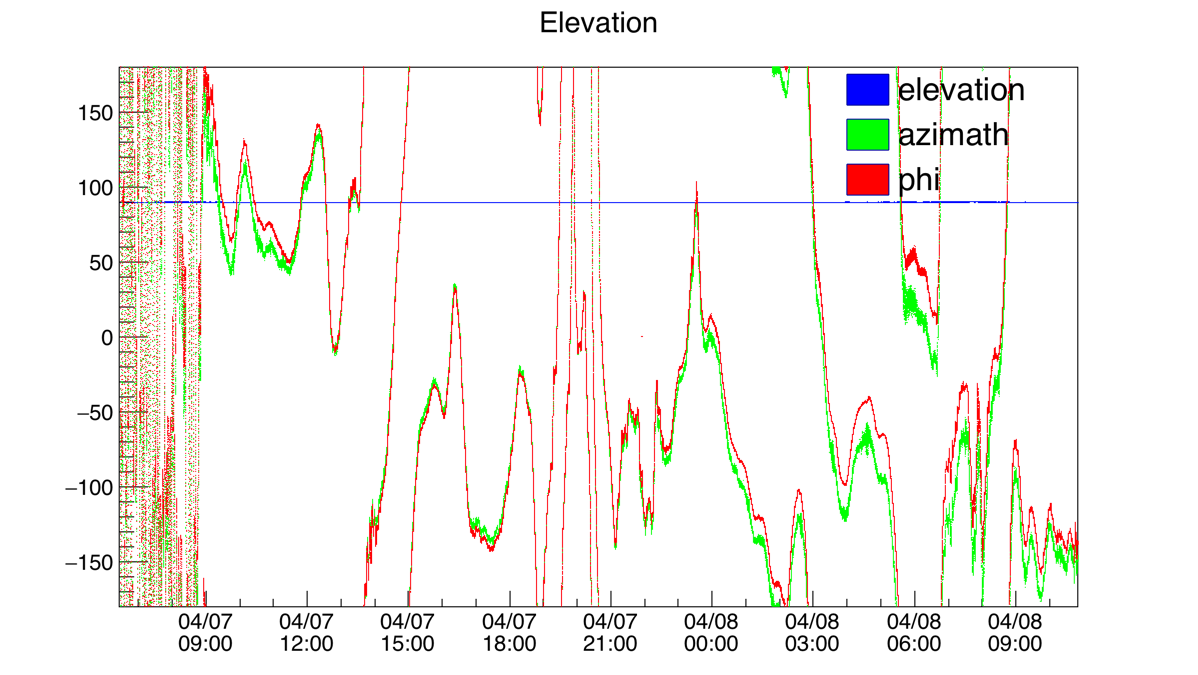
\includegraphics[width=15cm]{attitude_f.png}
\caption{test}
\end{figure}
